
\section{@@@ This marks the end of the reworked material}

\subsection{But what if you want source-code dependencies?}

But what if you really need a definition of semantic dependency
for a given code fragment that covers all executions?
One approach is to take the union of semantic dependencies across
all executions, so that if any execution has a semantic dependency,
the source code fragment has a semantic dependency.
This approach might be useful when carrying out static analysis.

On the other hand, many C++ implementations carry out specialization
optimizations, which consider groups of executions.
For example, an implementation might special-case a \co{NULL} pointer when
considering several inline functions that take early exits in that case.
For another example, an implementation might produce separate code for
cases where an integer is negative, zero, and positive.
Tools working with such implementations might therefore choose to group
executions by specialization, and then separately analyze semantic
dependencies for code corresponding to each specialize execution.

Other tools might need to take the intersection of semantic dependencies
across all executions, so that the source code fragment has a semantic
dependency only if all executions have a semantic dependency.
This approach might be useful when analyzing ordering properties
of that code fragment.

Nevertheless, in general, sdep must be defined on a per-execution basis.

\subsection{Where Do Loaded Values Come From?}
\label{sec:Where Do Loaded Values Come From?}

Relying on any rf link, whether the intra-thread rfi links or the
inter-thread rfe links, raises the question of what restrictions
might apply to C++ implementations' choice of value loaded.
For non-volatile atomic loads, this is question is answered by
the C++ standard in 6.9.2p14
\co{[intro.races]}~\cite{ThomasKoeppe2023N4950}:

\begin{quote}
	The value of an atomic object M, as determined by evaluation B,
	shall be the value stored by some side effect A that modifies M,
	where B does not happen before A.
\end{quote}

This wording presumably includes the initial value of M as one of the
possible side effects.
This means that an implementation might determine that a given atomic
object always has a given value, and such an implementation might
skip the load in favor of that value.\footnote{
	There is some work starting to forbid the implementation
	from using this assumption, for example, by requiring that
	the implementation assume that there is at least one thread
	that it does not know about.
	\url{https://hackmd.io/@gonzalob/Bk_ufPZ6o/edit}}

Please note that this does not apply to volatile atomic objects,
for which the implementation is prohibited from assuming that the
value loaded has any relationship whatsoever to any initialization
or any values stored.
This prohibition may come as a surprise to those carefully reading the
C++ standard~\cite{ThomasKoeppe2023N4950}
and finding only this wording constraining volatile accessess in
4.1.2p6
\co{[intro.abstract]}:

\begin{quote}
	Accesses through volatile glvalues are evaluated strictly
	according to the rules of the abstract machine.
\end{quote}

Unfortunately, volatile semantics are mostly folklore passed by word
of mouth among some compiler writers and some device-driver developers.
The key point is that volatile accesses must interact with MMIO
registers in such a way as to permit device drivers to be written.
And until such time as the semantics of all MMIO registers of all
devices have been formalized, published, and incorporated into
C++ implementations,\footnote{
	Given that some CPU vendors have started publishing formal
	memory models, this happy day might actually arrive.
	But we strongly recommend against holding your breath while
	waiting for it.}
these implementations cannot asssume that they can predict the value
returned by a volatile load.

\subsection{On OOTA Definitions}
\label{sec:On OOTA Definitions}

The earliest work defines ``OOTA cycle'' by example, without a precise
definition.
Sometimes ``causal cycle'' is used as if it was a definition, but
without a clear decision thread for what does and does not
constitute a causal cycle.
P0442R0 defines an OOTA cycle as a fixed-point computation that is
destroyed by perturbations, which makes perfect sense to that paper's
authors, but has left others unsatisfied.
Still others argue (perhaps correctly) that it is impossible to provide
a general definition of ``OOTA cycle'', but this simply raises
the question of whether a \emph{useful} definition can be formulated.

@@@ The C++ standard says this in 33.5.4p8
(\co{[atomics.order]})~\cite{ThomasKoeppe2023N4950}:

\begin{quote}
	Implementations should ensure that no “out-of-thin-air” values
	are computed that circularly depend on their own computation.
\end{quote}

The following sections discuss properties of and constraints on
useful definitions of ``semantic dependency''.

\subsubsection{@@@ Semantic Dependencies Are Per Execution}
\label{sec:Semantic Dependencies Are Per Execution}

\subsubsection{@@@ Semantic Dependencies Depend on Context}
\label{sec:Semantic Dependencies Depend on Context}

\subsubsection{@@@ Semantic Dependencies Can Be Nondeterministic}
\label{sec:Semantic Dependencies Can Be Nondeterministic}

\subsubsection{Semantic Dependencies And Optimization}
\label{sec:Semantic Dependencies And Optimization}

@@@ What do we do with this one???  Not sure we need it.

Consider again the following:

\begin{quote}
\begin{verbatim}
x = y + z;
\end{verbatim}
\end{quote}

Suppose that the implementation can prove that at any time that
the above statement might execute, \co{y} is equal to \co{z}.
That would allow the implementation to optimize, that is, to act as if
the source code was instead as follows:

\begin{quote}
\begin{verbatim}
x = 2 * y;
\end{verbatim}
\end{quote}

Or equally valid:

\begin{quote}
\begin{verbatim}
x = 2 * z;
\end{verbatim}
\end{quote}

In this case, is the semantic dependency from \co{y} to \co{x},
from \co{z} to \co{x}, or both \co{y} and \co{z} to \co{x}?
The answer is that this is a free choice on the part of the
implementation.
Those wishing to change the value of \co{y} or \co{z} externally
(for example, using a debugger) would do well to avail themselves
of the \co{volatile} keyword.

\emph{Semantic dependencies can be a free choice on the part of the
C++ implementation.}

\subsubsection{Semantic Dependencies and I/O}
\label{sec:Semantic Dependencies and I/O}

@@@ Not sure we need this one.

A computation might include I/O:

\begin{quote}
\begin{verbatim}
x = y * input_int();
\end{verbatim}
\end{quote}

Then there is a semantic dependency from \co{y} to \co{x} only if
the number input is non-zero.
Similar issues arise when reading timestamps.

In addition, I/O operations are observed behavior, which greatly restricts
optimizations involving them, in turn reducing the need to evaluate
potential semantic dependencies.

\subsubsection{@@@ Semantic Dependencies Can Be Complex}
\label{sec:Semantic Dependencies Can Be Complex}

\subsubsection{@@@ Implementers and Users Influence Semantic-Dependencies Definition}
\label{sec:Implementers and Users Influence Semantic-Dependencies Definition}

\subsubsection{Complex Semantic Dependencies Analysis is a Choice}
\label{sec:Complex Semantic Dependencies Analysis is a Choice}

All of these tools can incur high overhead, especially manual code
inspection.
However, as we will see, the actual C++ implementations themselves need
not use these tools.
Their current analysis is guaranteed to be sufficient, courtesy of the
real-world constraints discussed in the next section, at least assuming
that their analysis is in fact correct.
Furthermore, as we will also see, in some special but commonly occurring
circumstances, there are much simpler methods that incur negligible overhead.

\section{How to Form an OOTA Cycle?}
\label{sec:How to Form an OOTA Cycle?}

Rather than look at how to prevent an implementation from forming an
OOTA cycle, this section instead looks at how to form one.
This will lead to the conclusion that a correct real-world C
implementation cannot form OOTA cycles,\footnote{
	Keep in mind that C does not have non-volatile atomic
	operations.}
and provide guidance on how to avoid OOTA cycles for non-volatile relaxed
atomics in C++ implementations.

Again, an OOTA cycle consists of loads from other threads' stores where
a given store's address or value depends on the value returned by
the corresponding thread's prior load.
All of the links from one thread to the next are reads-from links, which
are temporal in nature, that is, a given store must execute earlier in
global time than any load from that stored-to object that returns the
value stored.

But it is also the case that an OOTA cycle must have at least one link
that goes backwards in time.
Given that the inter-thread links are temporal with a give store preceding
any load returning the value stored, the only possible candidate atemporal
links are those confined to a given thread.
This in turn requires that a store that depends on an earlier load
be executed earlier in time than that load.
The two ways that this can happen are when the implementation:

\begin{enumerate}
\item	Is able to prove the location and value of the store.
\item	Guesses the location and value of the store and has some means
	to take corrective action should any guess prove incorrect.
\end{enumerate}

Each of these possibilities is discussed in the next sections.
followed by a section on the possibility of flattening a multithreaded
program into a single thread.

\subsubsection{Executions Can Be Merged}
\label{sec:Executions Can Be Merged}

Consider this example, similar to that shown in
Section~\ref{sec:Semantic Dependencies Not Affected by if Statements},
which appears to be an \co{if} statement:

\begin{quote}
\begin{verbatim}
r1 = x;
if (r1 > 0)
    y = 42;
else
    y = 42;
\end{verbatim}
\end{quote}

Because the stores executed on each branch of that \co{if} statement store
identical values to identical addresses, one could equally well regard
the two statements as performing two different stores or as performing
(for all intents and purposes) a single store.
Although software projects relying on ordering from load-to-store control
dependencies and using a variety of compilers should should err on the
side of caution by assuming there is no semantic
dependency~\cite{Howells2009membartxt},
the fact remains that reasonable C++ implementations might disagree as
to whether this code represents one execution or two.
It is the implementations's choice.

A similar caution applies to loads:

\begin{quote}
\begin{verbatim}
r1 = x;
if (r1 > 42)
    r2 = y;
else
    r2 = y;
z = r2;
\end{verbatim}
\end{quote}

The two loads from \co{y} are fungible, and so a C++ implementation
could behave as if this \co{if} statement had instead been a single load
from \co{y}.

These examples demonstrate a key point: 
\emph{In general, executions do not necessarily map one-to-one onto
paths through the source code}.% \footnote{
% 	Thanks to Alan Stern for the examples in this section and
% 	in the preceding one.}

\subsubsection{Executions Depend on Context}
\label{sec:Executions Depend on Context}

Consider the following example derived from that in
Section~\ref{sec:Semantic Dependencies and Source Code}:

\begin{quote}
\begin{verbatim}
r1 = x;
// r1 = 0;
z = y * r1;
// z = y / r1;
\end{verbatim}
\end{quote}

As written, there is a semantic dependency from \co{x} and \co{y}
to \co{z}.
But if the second line is uncommented, there is no semantic
dependency.
If the second line is left commented, but the last line is uncommented,
then the compiler is free to backwards-propagate the potential
divide-by-zero undefined behavior to precede the first assignment
to \co{z}.
This could prevent both assignments to \co{z} from executing, for example,
due to a divide-by-zero exception.

More subtle changes in context can also have an effect.
For example:

\begin{quote}
\begin{verbatim}
r1 = x;
z = y * r1;
z = 42;
\end{verbatim}
\end{quote}

Given that there is no ordering, a C++ implementation could choose to
act as if the first store to \co{z} was omitted, even if that store was
a relaxed atomic store.
But if \co{z} was marked volatile, both stores would need to be executed
in strict accordance with the rules of the abstract machine.

\emph{Any analysis of a given execution either must be fully informed
of the enclosing context, or must make conservative assumptions about
that context.}

\subsubsection{Executions Can Be Nondeterministic}
\label{sec:Executions Can Be Nondeterministic}

Consider this example, similar to that in
Section~\ref{sec:Abstract Executions},
with \co{i} initially zero:

\begin{quote}
\begin{verbatim}
int foo(int a, int b)
{
   return a / b;
}

y = foo(++i, ++i);
x = y * z;
\end{verbatim}
\end{quote}

Because early C~implementers could not come to agreement, standard
does not specify the order of evaluation of function arguments, so the
resulting value of \co{y} might be zero ($\frac{1}{2}$ truncated) or two
($\frac{2}{1}$).
In the former case, there is no semantic dependency from \co{z} to
\co{x}, but in the latter case there is.
Thus, semantic dependencies are not just a function of a particular
execution through the source code, but also of arbitrary choices made
by the C++ implementation.\footnote{
	Again, thanks to Peter Sewell for pointing out this possibility.}

Note well that C++ implementations can and do act as if portions of
the source code was duplicated in order to apply specialization
optimizations, in which case any non-determinism might also be
a function of a given execution.

Many projects' coding guidelines prohibit side effects in expressions,
their goal being to obtain portable code whose behavior does not depend
on arbitrary choices on the part of the implementation.
However, the above code nevertheless conforms to the standard.
Note that side effects in expressions lacking sequence points is
undefined behavior, however, there are proposals to define it in the
C++~\cite{GabrielDosReis2016P0145r3} and
C~\cite{AlexCeleste2023N3203}
languages, allowing implementations to nevertheless reorder
evaluation when permitted by the as-if rule.

Even though the standard is non-deterministic, \emph{compiler-based C++
implementions make their non-deterministic choices at compile time, so
that the object code is deterministic, at least on a per-execution basis.}

\subsubsection{Implementers and Users Influence the Definition of Execution}
\label{sec:Implementers and Users Influence the Definition of Execution}

The exact definition of a computer language is subject to some debate,
with standards, implementations, and users all having some degree of
influence~\cite{KayvanMemarian2016DepthOfC-1,KayvanMemarian2016DepthOfC-2},
and each of which is subject to change over time.
Users  and implementers are of course wise to assume that their opinions
might be overridden by those of the standard and, for the users,
especially the implementation.
However, consider the following code, similar to that shown in
Section~\ref{sec:Abstract Executions}:

\begin{quote}
\begin{verbatim}
void foo(int x, char c)
{
    return x * (c >= 0);
}
\end{verbatim}
\end{quote}

The standard does not specify whether or not type \co{char} is signed,
leaving that choice to the implementations, which follow the lead
of the architects of a given CPU family.
Therefore, the code above has a semantic dependency in executions running
on systems choosing signed \co{char}, but not those running on systems
choosing unsigned \co{char}.
So score one for the implementers, albeit by conscious choice on the
part of the standards committee.

Except that GCC provides the \co{-funsigned-char} command-line
argument that causes this implementation to treat variables of
type \co{char} as unsigned, regardless of the architects' wishes.
Given this command-line argument, there is always a semantic dependency
in the execution running from the \co{foo()} function's argument to its
return value.
So score one for at least some implementations' users.

Please see Appendix~\ref{app:User Influence Over Language Semantics}
for more examples of user control over semantics, including semantic
dependencies.

\emph{A definition of ``execution'' drawn strictly from the standard will
be at best an approximation to a definition that is useful in practice.}

\subsubsection{So What Exactly is an Execution, Anyway?}
\label{sec:So What Exactly is an Execution, Anyway?}

Given all of these complications in C++ executions, and given that
semantic dependencies must be defined in terms of executions, it makes
sense to lower our sights from full generality.
We therefore restrict ourselves to a specific context:
traditional compilers.
It will then turn out to be necessary to take the notion of semantic
dependence, and thus OOTA, to be compiler-relative rather than absolute.

We will show that programs built using loose C++ compilers that treat all
atomic operations as volatile can never exhibit OOTA, and the same is true
for compilers obeying the weaker constraint that atomic accesses may not
invented, provided the compiler does not perform multi-thread analysis.

% @@@ LTO?  Does not appear to be relevant given new material.

These restrictions permit us to bring to bear the real-world
constraints introduced by the next section.

\subsection{Implementation Proves Value}
\label{sec:Implementation Proves Value}

Implementation can sometimes prove the location and value of a given
store.
For example, if the value loaded is multiplied by zero, the result
is known to be zero, so that the store can proceed prior to the load.
But in this case, there is no way that the value returned from
the load that can affect the value stored.
Therefore, that store cannot possibly take part in an OOTA cycle.

\subsection{Implementation Guesses at Value}
\label{sec:Implementation Guesses at Value}

Hardware speculative execution is commonplace, and permits the
hardware to guess at values, squashing the speculation if any
of the guesses prove incorrect.
But in this case, a given store is not committed until all guesses that
this store depends on have been confirmed, and thus no uncommitted store
is visible to any other thread.
Therefore, any hardware speculation that results in OOTA cycles is doomed
to be squashed an discarded, and by design, even on weakly ordered
systems~\cite{ARMv7A:2010,ARMv8A:2017,PowerISA2.07-2013}.
This same constraint applies to software, which might use compare-and-swap
loops or hardware transactional memory to confirm guesses.

Either way, the need to wait for guesses to be confirmed before committing
stores prevents those stores from becoming visible prior to the
completion of any loads that those stores depend on.

\subsection{But What About Flattening?}
\label{sec:But What About Flattening?}

The concept of flattening multiple threads into a single thread is
tantalizing, especially given the large cache-miss penalties inherent
to large multicore systems, which can have many sockets containing
thousands of CPUs.
One might object to the whole concept of flattening as an
optimization given the difficulty inherent in avoiding deadlocks
and other hazards.
Nevertheless, it is only reasonable to ask whether flattening can
result in OOTA cycles.
As we will see, the answer is ``no''.

The reason for this answer is that any fully flattened program will be
single threaded, which implies that each of its atomic load operations
will return the last value stored to that same object in sequenced-before
order (or the initial value if there is no such store).
Thus, any sequence of loads and stores must have a first operation and
a last operation, and the last operation cannot affect the first
operation.
Therefore, cycles cannot possibly form in a flattened program,
which in turn implies that OOTA cycles cannot form.

\subsection{But What About Non-Volatile Atomics?}
\label{sec:But What About Non-Volatile Atomics?}

Volatile atomic accesses have some very attractive properties from
the viewpoint of analyzing executions for OOTA behavior because C++
compilers are prohibited from reordering, omitting, fusing, or inventing
volatile accesses.
Thus, if the compiler emits code that faithfully reflects the behaviors
specified by the source code, the hardware memory model will prohibit
OOTA cycles.

However, there is some question as to what exactly a C++ implementation
is permitted to do with non-volatile atomic accesses~\cite{JFBastien2015N4455}.
For example,
Appendix~\ref{app:Inventing Atomic Loads}
shows a clever litmus test that results in OOTA-like behavior
if a C++ implementation duplicates an atomic load, compares the two values
loaded, and then, if the two loads return different values, chooses the
one that eliminates a semantic dependency that would otherwise remain
in place.
Perhaps in the fullness of time, such examples will be considered to be
simple optimizations rather than full-on OOTA cycles, but in the meantime
C++ implementations might wish to prohibit such behavior.

Keeping in mind that some early C++ implementations treated non-volatile
atomic operations as if they were volatile, one way to accomplish this
while still permitting optimization of code containing non-volatile
atomics is to model non-volatile behavior on that of volatile atomics,
but with some specific weakenings, for example:

\begin{itemize}
\item	Loads that do not affect observable behavior can be omitted,
	along with any computations based on their return values.
\item	Given a pair of loads from the same object that can be
	reordered to be adjacent to each other, if one of the pair is a
	relaxed load, it can be omitted, with uses of the omitted load
	instead using the value returned by the surviving load.
	This is termed \emph{load fusing}.
\item	Given a pair of stores to the same object that can be reordered
	to be adjacent to each other, if the first of the pair is a
	relaxed store, it can be omitted.
	This is termed \emph{store fusing}.
\item	Suppose the source code contains a pair of non-volatile atomic
	loads from objects that are adjacent in memory.
	Suppose further that these loads can be reordered to be adjacent
	to each other, and that the last of the two is a relaxed load.
	Then this pair of loads can be replaced with a single load
	from both objects using the first load's memory order.
	This is termed \emph{load consolidation}.
\item	Suppose the source code contains a pair of non-volatile atomic
	stores to objects that are adjacent in memory.
	Suppose further that these stores can be reordered to be adjacent
	to each other, and that the first of the two is a relaxed load.
	Then this pair of loads can be replaced with a single store
	to both objects using the last store's memory order.
	This is termed \emph{store consolidation}.
\item	If an expression can be proven to always result in a constant,
	that constant can be substituted for that expression.
	Note well that combining this with specialization optimizations
	can convert address and data dependencies to weaker control
	dependencies.
	Address and data dependencies order later loads and stores,
	and control dependencies order only later stores.\footnote{
		Yes, yes, the C++ standard does not mention address or
		data dependencies, and mandates control dependencies
		only indirectly (via the prohibition against introducing
		data races).
		Such dependencies nevertheless still exist.}
\end{itemize}

Note that load and store fusing can only be applied a finite number of
times.
In practice, this means that fusing can be used to unroll loops, but
not to hoist atomic loads or stores out of loops than cannot be proven
to be always finite.

Note also that many users would consider it to be an extremely unfriendly
act for a C++ implementation to combine loads or stores to adjacent
objects where each object \co{is_lock_free()}, but the combination is not.

These optimizations are examples, not necessarily a full set.
Additional optimizations might be added over time, but great care will
of course be required.

\subsection{But What About Multi-Threaded Optimizations?}
\label{sec:But What About Multi-Threaded Optimizations?}

Although this paper mostly ignores multi-threaded implementations,
JMM Causality Test Cases 1, 8, 9, and 9a discuss inter-thread
analysis or constraints on thread scheduling.
This topic is therefore worth a short discussion.

In order to set context, it is important to note that an oracular C++
implementation could in theory read a program and its input, and then
perform a sequence of observable behaviors consistent with that program
running on that input without actually executing that program's code.
This admittedly extreme example shows that it is not unreasonable to
impose some real-world constraints on a real C++ implementation, and
limiting analysis to a single thread is one of the constraints that we
have chosen.

At the same time, it is worth calling out some optimizations based on
multi-threaded analysis that can be introduced without risk of
introducing OOTA cycles.

First, given a variable that the implementation can prove is always equal
to some constant, the implementation may act as if the program's uses of
that variable's value instead used that constant.

Second, given a pair of variables that the implementation can prove always
have a given algebraic relation to each other, the implementation can
act as if that program's uses of one of the variable's values instead
used the corresponding function of the other variable's value.
However, if the values of those variables are subject to change, there
must be some form of synchronization in effect to prevent accesses
to those variables' values during times when a given modification has
changed the value of one of the variables but not yet that of the other.
If there is no such synchronization, then this optimization cannot
be applied.

Third, given that the implementation can prove that one thread always
terminates before another thread starts, and if one or another of the
threads does nothing related to thread identity, the implementation
may act as if these two threads had been fused into a single thread.

Fourth and finally, if the implementation can prove that a given thread
never executes, the implementation may act as if code specific to that
thread had been omitted from the program.

Although these last two examples might appear to be a bit utopian,
the first two provide ample room for multi-threaded analysis.

\subsection{Correct Implementations Cannot Form OOTA Cycles}
\label{sec:Correct Implementations Cannot Form OOTA Cycles}

This section has shown that an implementation that correctly handles
the memory model, observable behavior, and the as-if rule cannot form
OOTA cycles from volatile atomics when running UB-free programs on real
systems in this universe.
It has also presented a substantial list of optimizations that can be
applied to non-volatile atomics without the risk of creating OOTA cycles.

\clearpage

\section{Aside on Undefined Behavior}
\label{app:Aside on Undefined Behavior}

The combination of OOTA cycles and UB has proven especially
challenging~\cite{DavidGoldblatt2019NoElegantOOTAfix,HansBoehm2020UBalternatives}.

\subsection{Alignment-Based Undefined Behavior}
\label{sec:Alignment-Based Undefined Behavior}

The example shown in
Listing~\ref{lst:Alignment-Based Undefined Behavior (P1916R0)}
(taken from P1916R0) is especially instructive.

\begin{listing}[tbp]
\begin{verbatim}
 1 std::atomic<int> y;
 2 template <typename T>
 3 void t1() {
 4   long long r1 = x.load(std::memory_order_relaxed);
 5   if (r1 % 4 == 0)
 6     y.store(1, std::memory_order_relaxed);
 7   *(T*)r1 = *(T*)r1;
 8 }
\end{verbatim}
\caption{Alignment-Based Undefined Behavior (P1916R0)}
\label{lst:Alignment-Based Undefined Behavior (P1916R0)}
\end{listing}

Because the compiler often assumes that UB cannot happen, it might
look at line~7 and conclude that the value of \co{r1} necessarily
corresponded to an address aligned per the requirements of type \co{T}.
If that type's alignment was larger than four bytes, the compiler could
then replace the condition in line~5 with \co{true}, which would mean
that there was no semantic dependency from the load of \co{x} to the
store of \co{y}.

Except that the developer might have knowingly carried out a misaligned
access, for example, to test an alignment trap handler or because the
system on which this code was to run was known to gracefully handle
misaligned accesses.

\begin{listing}[tbp]
\begin{verbatim}
 1 std::atomic<int> y;
 2 template <typename T>
 3 void t1() {
 4   long long r1 = x.load(std::memory_order_relaxed);
 5   if (r1 % 4 == 0)
 6     y.store(1, std::memory_order_relaxed);
 7   std::observable();
 8   *(T*)r1 = *(T*)r1;
 9 }
\end{verbatim}
\caption{Alignment-Based Undefined Behavior Fix}
\label{lst:Alignment-Based Undefined Behavior Fix}
\end{listing}

However, in that case, the developer is stepping outside the bounds
of the standard.
It would be good to have some way for the developer to get the job
done without confusing the compiler, thus separating OOTA-cycle and
UB concerns.
One approach is to use the \co{std::observable()} function
that has been proposed to the C++ standards
committee~\cite{DavisHerring2021P1494R2}.
This function would blocks backwards-propagating UB.
Then this example could be rewritten as shown in
Listing~\ref{lst:Alignment-Based Undefined Behavior Fix},
with the asm on line~7 preventing the compiler from assuming that line~8
is guaranteed to be executed, thus preventing the compiler from
applying any lessons that it might learn from line~8 to line~5.

% Clean up <200b> in vim: ":%s/\%u200b//g"

There are a number of ways to implement \co{std::observable()},
for example, a new \co{"mightnotreturn"} GCC asm clobber, a call to an empty
function that is invisible to the compiler, and a GCC goto asm that the
compiler cannot prove falls through.\footnote{
	Rust defines non-pure asms as potentially looping forever.
	\url{https://github.com/rust-lang/reference/pull/1442}}

\subsection{Unreachability-Based Undefined Behavior}
\label{sec:Unreachability-Based Undefined Behavior}

This section attempts to apply the lessons
of Appendix~\ref{sec:Unreachability-Based Undefined Behavior} to
Goldblatt's unreachability-UB example.

The \co{std::observable()} at line~12 of
Listing~\ref{lst:Alignment-Based Undefined Behavior Fix}
avoids confusing the compiler, instead forcing it to assume that the
value of \co{local} might not be zero.

\begin{listing}[tbp]
\begin{verbatim}
 1 // UB if this function is ever called.
 2 [[noreturn]]
 3 inline void unreachable() {
 4   return;
 5 }
 6 void t1() {
 7   r1 = x.load(std::memory_order_relaxed);
 8   int local = (r1 & 1);
 9   if (local == 0)
10     y.store(1, std::memory_order_relaxed);
11   if (local != 0) {
12     std::observable();
13     // If we get here, UB.
14     unreachable();
15   }
16 }
\end{verbatim}
\caption{Unreachability-Based Undefined Behavior Fix}
\label{lst:Unreachability-Based Undefined Behavior Fix}
\end{listing}

By the same reasoning, Goldblatt's \co{misbehave} example that
also involves unreachability can also be addressed through insertion
of the proposed \co{std::observable()}.

\subsection{Atomic Stores From Undefined Behavior}
\label{sec:Atomic Stores From Undefined Behavior}

Another proposal to the C++ standards
committee~\cite{HansBoehm2020UBalternatives}
proposes (among other alternatives) that any atomic store resulting
from undefined behavior have at least release semantics.
This would prevent such a store from propagating undefined behavior
backwards within that store's thread.
In some cases, this could also prevent this undefined behavior from
propagating back through other threads.

However, it might well force C++ implementations to promote a surprisingly
large fraction of a program's relaxed stores to release.

\subsection{Lifetime-Based Undefined Behavior}
\label{sec:Lifetime-Based Undefined Behavior}

Not all undefined behavior can be backstopped using
\co{std::unreachable()}.

\begin{listing}[tbp]
\begin{verbatim}
 1 int *foo(int *r)
 2 {
 3   b.store(r, memory_order_relaxed);
 4   return &global;
 5 }
 6
 7 int go(int *p)
 8 {
 9   int r;
10   int *q = foo(&r);
11
12   r = 2;
13   *p = 1;
14   *q = r;
15   return *q - r;
16 }
17
18 void t1(void)
19 {
20   int r1 = go(a.load(memory_order_relaxed));
21   printf("go() = %d\n", r1);
22 }
23
24 void t2(void)
25 {
26   int *r2 = b.load(memory_order_relaxed);
27   a.store(r2, memory_order_relaxed);
28 }
\end{verbatim}
\caption{Lifetime-Based Undefined Behavior}
\label{lst:Lifetime-Based Undefined Behavior}
\end{listing}

Listing~\ref{lst:Lifetime-Based Undefined Behavior}
shows an example loosely based on one presented by Stephen Dolan\footnote{
	\url{https://stedolan.net/talks/2024/loadstore}}
in which function \co{go()} invokes \co{foo()} with a pointer to \co{go()}'s
local variable \co{r}.
However, \co{foo()} uses a relaxed store to place this pointer in
an atomic variable \co{b}.
Because this store is relaxed, it is not ordered against other code
in \co{go()} and \co{t1()}, which means that \co{t2()} might well
read this pointer from \co{b} either before the beginning or after
the end of \co{r}'s lifetime, neither of which is well-defined.

Of course, any attempt to dereference the pointer read from either
\co{a} or \co{b} could result in undefined behavior.

The lesson is clear:
Properly synchronize reads and writes of pointers with the lifetime
of the pointed-to object.

This example could make lines~3 and~27 be \co{memory_order_release} and
lines~20 and~26 be \co{memory_order_acquire} in order to avoid carrying
a pointer to \co{r} before the lifetime of \co{r} has started.
Alternatively, threads could be spawned only after \co{r}'s lifetime
starts and joined before it ends.
Placing \co{r} in static global storage would avoid lifetime considerations
totally.
And there are of course any number of other synchronization schemes
that might be used to ensure that pointers are in use only while the
pointed-to objects are alive.

Note that \co{std::unreachable()} does not suffice because the CPU
can also reorder relaxed stores.
Note also that load-store ordering is not sufficient to prevent a
pointer to \co{r} from being stored to \co{b} prior to the start of
\co{r}'s lifetime because there is no atomic load between the start
of that lifetime and the relaxed store to \co{b}.

There are a number of ways to prevent carrying a pointer to \co{r} after
the lifetime of \co{r} has ended, and these are left as an exercise for
the reader.

\clearpage

\section{Evaluating sdep Using \co{cbmc}}
\label{sec:Evaluating sdep Using cbmc}

This section demonstrates the evaluation of sdep using
the C Bounded Model Checker
(\co{cbmc})~\cite{EdmundClarke2004CBMC}.
This tool takes a smallish C program as input and constructs a logic
expression representing that program.
The logic expression's variables represent bits in the program's inputs
and state, and the result of that logic expression is \co{true} if that
program has a bug, for example, if it is possible for that C program to
trigger an assertion or execute an out-of-bounds array reference.
The tool then hands this expression to a SAT solver, and if this solver
finds a satisfying set of values, the tool uses those values provide
the execution path to the bug.

But first, Appendix~\ref{app:Informal Definition of Semantic Dependency}
outlines an informal informal definition of ``semantic dependency''
that can be used in \co{cbmc} test cases, and then
Appendix~\ref{sec:Executions Can Be Complex} gives some examples
of mathematically complex semantic dependencies.

\subsection{Informal Definition of Semantic Dependency}
\label{app:Informal Definition of Semantic Dependency}

The manual analysis uses the informal rule that a semantic dependency
exists between a set of relaxed atomic loads\footnote{
	Please see
	Appendix~\ref{app:Non-Trivial Semantic Dependencies}
	for examples showing why this is a set of loads rather than a
	single load.}
and a store on any execution where different values loaded would change
the address stored to, the value stored, or the number of times that
store would be executed, with the proviso that stores of the same value
to the same address having the same ordering properties are fungible.

Producing a precise formal statement of this rule turns out to be quite
challenging, but as noted earlier, there is considerable work along
various
lines~\cite{Lahav:2017:RSC:3062341.3062352,Sinclair:2017:CAR:3079856.3080206,Lee:10.1145/3385412.3386010,MarkBatty2019ModularRelaxedDependenciesOOTA}.
For examples of the challenges, please see
Section~\ref{sec:On OOTA Definitions}.
Our informal definition meets these challenges as follows:

\begin{enumerate}
\item	Section~\ref{sec:Semantic Dependencies and Source Code}
	is responsible for the phrase ``on any execution'' as well
	as the proviso regarding fungible loads.
\item	Section~\ref{sec:Semantic Dependencies Depend on Context}'s
	challenges are met by looking at the full context within
	a given thread.
\item	Section~\ref{sec:Semantic Dependencies Can Be Nondeterministic}'s
	non-determinism challenges are avoided by avoiding litmus tests
	exhibiting non-deterministic behavior.
	Again, note that most production C++ code uses compiler-based C++
	implementations, which freeze their non-deterministic choices
	into the binary at compile time.
\item	Section~\ref{sec:Semantic Dependencies And Optimization}'s
	optimization-choice challenges are met by using the C++
	implementation's choice of semantic dependency based on the
	optimizations that the implementation actually applied.
\item	Section~\ref{sec:Semantic Dependencies and I/O}'s
	I/O challenges are met by again noting that I/O is observed
	behavior.
	And by avoiding litmus tests involving I/O, given that relatively
	few of the available tools handle I/O.
\item	Section~\ref{sec:Semantic Dependencies Can Be Complex}'s
	complexity challenges are met by looking at what the code
	actually does.
	For example, if an as-yet unproven mathematical conjecture
	holds, the code will act consistently with that conjecture,
	and vice versa.
\item	Section~\ref{sec:Implementers and Users Influence Semantic-Dependencies Definition}'s
	implementer-/user-choice challenges are met by accounting for
	those choices.
	For example, if a user has specified \co{-funsigned-char},
	then the actual executions will be consistent with that choice.
	For more examples, please see
	Appendix~\ref{app:User Influence Over Language Semantics}.
\end{enumerate}

In short, we are treating ``semantic dependency'' in a manner similar
to our treatment of the laws of physics.
We let the actual executions provide an empirical basis for the analysis.

We do not expect this approach to please everyone.
However, those who are displeased might do well to reflect on the fact
that the C++ standard is not mathematical in nature, which implies that
any mathematical model of C++ is inherently an approximation.
We look forward to the day when the standard gains more mathematical
rigor, and perhaps the C++ memory model is a first step in that
direction.\footnote{
	But if so, the OOTA situation should be a caution!}
Nevertheless, until that day, we must live with the standard in its
current decidedly non-mathematical form.

\subsection{Executions Can Be Complex}
\label{sec:Executions Can Be Complex}

Consider this example:

\begin{quote}
\begin{verbatim}
x = horribly_complex(y, z);
\end{verbatim}
\end{quote}

Here, the presence or absence of a semantic dependency from \co{y} to
\co{x} depends not only on the value of \co{z}, but also and execution
that passes through the code in a function that, although single threaded,
is horribly complex.

A special case is as follows:

\begin{quote}
\begin{verbatim}
x = y & 0x1 ? do_odd(y) : do_even(y);
\end{verbatim}
\end{quote}

The key point here is that different values might result in almost
completely disjoint executions.

Fortunately, there are now tools that can help.
For example, the SAT-solver-based \co{cbmc} tool
has been used to mechanically verify signicant portions of Linux-kernel
RCU from the C-language source
code~\cite{LihaoLiang2016VerifyTreeRCU,LanceRoy2017CBMC-SRCU}.
Another tool, Nidhugg, which is based on partial-order
reduction, has been used to carry out a similar
verification~\cite{MichalisKokologiannakis2017NidhuggRCU,SMC-TreeRCU,MichalisKokologiannakis2019RCUstatelessModelCheck}.
Both tools can easily check whether or not a given dependency is semantic
for at least some approximate definitions of ``semantic dependency''.
% An example use of \co{cbmc} is illustrated in
% Appendix~\ref{sec:Evaluating sdep Using cbmc}.

There are also many other tools, but failing that, it is always possible
to fall back to older software-verification tools such as manual
code inspection.

But consider the following code fragment:

\begin{quote}
\begin{verbatim}
x = collatz_cycle_min(y);
\end{verbatim}
\end{quote}

Here, \co{collatz_cycle_min()}\footnote{
	\url{https://en.wikipedia.org/wiki/Collatz_conjecture}}
takes its arbitrary-precision-integer argument and repeatedly either
divides it by two if it is even, or multiplies it by three and adds one
if it is odd.
Should the resulting sequence of arbitrary-precision integers reach
a cycle, the function returns the minimum element of that cycle.
Leaving aside the practical complication of a value of \co{y} that
consumes more than half of the available memory, there is reason to
believe that the above code fragment will always assign the value 1 to
\co{x}.
Except that this reason for belief is based on the Collatz conjecture,
which is currently unproven and might never be proven (or disproven).

A similar example could be constructed from Fermat's Last Theorem
(FLT),\footnote{
\url{https://en.wikipedia.org/wiki/Fermat\%27s_Last_Theorem}}
which was first stated in the year 1637 and finally proved more than
300~years later, in 1994.
Therefore, it was only after 1994 that certain types of executions
relying on FLT were known not to have a semantic dependency.

Many analysis tools would respond to these examples by failing, for example,
by consuming all available CPU and memory.

One could quite reasonably argue that these two examples are irrelevant
to any real-world C++ implementation.
After all, evidence to date suggests that code relying on either the
Collatz Conjecture or FLT is quite rare, and thus not worth optimizing.
And the value of any given optimization is another real-world constraint
on the problem of locating OOTA cycles, but one that will not be considered
further in this document.

\emph{Because of unsolved mathematical problems, precise definitions of
``execution'' have limitations.
Therefore, C++ implementations must assume that a dependency passing
through a given execution is a semantic dependency unless and until it
can prove otherwise.}

\subsection{Complex Semantic Dependencies}
\label{app:Complex Semantic Dependencies}

Listing~\ref{lst:Example Code for Evaluation of sdep}
shows a \co{herd7} thread \co{P0()}.
Is there a semantic dependency between the load from \co{x} on
line~3 to the store to \co{y} on line~9?
Answering this question requires solving a mathematical equation,
not all of which currently have known solutions.
However, this section will use a relatively simple equation combined
with restrictions on domain and range that permit \co{cbmc} to do
the job.

\begin{listing}[tbp]
\scriptsize
\begin{verbatim}
 1 P0(atomic_int *x, atomic_int *y, atomic_int *limit)
 2 {
 3   r1 = atomic_load_explicit(x, memory_order_relaxed);
 4   r2 = atomic_load_explicit(limit, memory_order_relaxed);
 5   r3 = r1 * r1 + 2 * r1 + 2;
 6   r4 = r2;
 7   if (r2 >= r3)
 8     r4 = r3;
 9   atomic_store_explicit(y, r4, memory_order_relaxed);
10 }
\end{verbatim}
\caption{Example Code for Evaluation of sdep}
\label{lst:Example Code for Evaluation of sdep}
\end{listing}

\begin{listing}[tbp]
\scriptsize
\begin{verbatim}
 1 int main(int argc, char *argv[])
 2 {
 3   int i;
 4   int y[2] = { 0, 0 };
 5
 6   for (i = 0; i < 2; i++) {
 7     int r1;
 8     int r2;
 9     int r3;
10     int *yp = &y[i];
11
12     r1 = limited_arg(argv[2 * i + 1]);
13     r2 = const_arg(limited_arg(argv[2 * i + 2]));
14     r3 = r1 * r1 + 2 * r1 + 2;
15     *yp = r2 <= r3 ? r2 : r3;
16     printf("i = %d, r1 = %d, r2 = %d, r3 = %d\n", i, r1, r2, r3);
17   }
18   assert(y[0] == y[1]);
19 }
\end{verbatim}
\caption{Code for cbmc-Based Evaluation of sdep}
\label{lst:Code for cbmc-Based Evaluation of sdep}
\end{listing}

One way to answer this question is to create a C program
(see Listing~\ref{lst:Code for cbmc-Based Evaluation of sdep})
that runs the \co{P0()} thread's code twice with arbitrary inputs
(the loop spanning lines~6-17) and asserts that the results of
each iteration be equal (line~18).

Running this with:

\begin{quote}
\scriptsize
\begin{verbatim}
cbmc -DCBMC cbmc/sdep-quadratic.c
\end{verbatim}
\end{quote}

gives the result \co{VERIFICATION FAILED}.
This indicates that there are different values of \co{x} and \co{limit}
that yield different values of \co{y}, that is, that there can be
a semantic dependency.

\begin{listing}[tbp]
@@ DisplayLitmus cbmc/sdep-quadratic.c @@
\caption{Full Code for cbmc-Based Evaluation of sdep}
\label{lst:Full Code for cbmc-Based Evaluation of sdep}
\end{listing}

However, $x^2 + 2x + 2$ has a minimum value of 1 at $x=-1$, so
forcing \co{limit} to (say) zero should eliminate this static
dependency:\footnote{
	See Listing~\ref{lst:Full Code for cbmc-Based Evaluation of sdep}
	for the full \path{cbmc/sdep-quadratic.c} program.}

\begin{quote}
\scriptsize
\begin{verbatim}
cbmc -DCBMC -DLOAD_CONSTANT=0 cbmc/sdep-quadratic.c
\end{verbatim}
\end{quote}

But this also gives the result \co{VERIFICATION FAILED}.
One reason for this is that this program does 32-bit computer arithmetic,
and is thus subject to wraparound.
Limiting the value of \co{x} to 46,339 prevents wraparound:

\begin{quote}
\scriptsize
\begin{verbatim}
cbmc -DCBMC -DLOAD_CONSTANT=0 -DLOAD_LIMITS=46339 cbmc/sdep-quadratic.c
\end{verbatim}
\end{quote}

And this yields \co{VERIFICATION SUCCESSFUL}, indicating that there
is no semantic dependency in this case.
This is to be expected because the specified value of zero for \co{limit}
is smaller than the minimum of the quadratic expression, so that the
value stored to \co{y} is always zero.
Specifying \co{-DLOAD_CONSTANT=1} also yields \co{VERIFICATION SUCCESSFUL}
because this value is equal to that minimum, so that the value stored to
\co{y} is always 1.
However, specifying any larger value (for example, \co{-DLOAD_CONSTANT=2})
yields \co{VERIFICATION FAILED} because the value assigned to \co{y}
might be either 1 or 2, indicating that a semantic dependency exists.

This situation underscores the point that the existance of a semantic
dependency can be a property of a particular execution rather than a
universal property of the code itself.
The interested reader is encouraged to create more complex examples,
for example, demonstrating semantic dependencies from multiple loads or
exploring indeterminacy.

There are numerous other tools that can be used, up to and including
manual inspection, but \co{cbmc} is readily available and easy to
use.\footnote{
	On Debian-based distributions, via \co{sudo apt install cbmc}.}

\subsection{C++ Non-Determinism}
\label{app:C++ Non-Determinism}

The C++ standard allows non-determinism, for example, the order of
invocation of side-effects in some circumstances.
Listing~\ref{lst:Code for cbmc-Based Evaluation of Non-Deterministic sdep}
shows an example leveraging side-effects in the parameter list shown on
line~37.

\begin{listing}[tbp]
@@ DisplayLitmus cbmc/sdep-nondet.c @@
\caption{Code for cbmc-Based Evaluation of Non-Deterministic sdep}
\label{lst:Code for cbmc-Based Evaluation of Non-Deterministic sdep}
\end{listing}

Running \co{cbmc} on this as follows:

\begin{quote}
\scriptsize
\begin{verbatim}
cbmc -DCBMC cbmc/sdep-nondet.c
\end{verbatim}
\end{quote}

Gives the result \co{VERIFICATION SUCCESSFUL}, showing that \co{cbmc}
does not model this non-determinism.
Which is not surprising, given that many of the safety-critical uses
to which \co{cbmc} is put would prohibit such non-determinism in their
code bases.

\clearpage

\section{Debates on Causality}
\label{sec:Debates on Causality}

This Appendix is provided as a service to readers who want to know more
about the ongoing debates on causality, provided by the combined efforts
of Bard, Chat-GPT, and Bing Co-Pilot.
References may be found here:

{ \scriptsize
\url{https://docs.google.com/document/d/1MJ6pQ4TcWchUQvoI-qhLjdhPVYF14AytbTW3gr4-xag/edit?usp=sharing}
}

The concept of causality, the idea that events are caused by preceding
events in a predictable and consistent manner, is fundamental to many
scientific theories and our understanding of the world.
However, when it comes to the universe as a whole, particularly at the
most fundamental levels such as in quantum physics or the origins of
the universe, the idea of strict causality can become more complex.

In classical physics, causality is often described in terms of
deterministic laws, where events are determined by prior causes.
But at the quantum level, the behavior of particles can be probabilistic
and uncertain.
Quantum mechanics introduces a level of randomness and uncertainty that
challenges our classical notions of causality.

Additionally, when considering the origin of the universe (the Big Bang),
the laws of physics as we understand them break down at extremely high
densities and temperatures.
The conditions at the very beginning of the universe might not conform
to our classical understanding of causality, and some theories suggest
that time itself might have begun with the Big Bang, making it difficult
to define causality in a traditional sense within such a framework.

On the one hand, there is a strong case to be made that the universe
is causal.
Our understanding of physics is based on the principle of causality,
which states that every event has a cause.
This principle has been incredibly successful in explaining and predicting
the behavior of the universe at large scales.
Additionally, our own personal experience seems to confirm causality.
We constantly observe events being caused by other events, and we have
no reason to believe that this is an illusion.

However, there are also some challenges to the idea of a perfectly
causal universe.
One challenge comes from quantum mechanics, which suggests that some
events may be fundamentally non-causal.
For example, the collapse of a wave function in quantum mechanics seems
to be a random event, with no underlying cause.
Additionally, our understanding of the universe's origins is still
very limited.
We don't know whether the Big Bang itself had a cause, or whether it
was simply the beginning of everything.

In summary, while causality is a fundamental concept in our understanding
of the universe, its application and implications can become more complex,
especially at the quantum level and regarding the origin of the universe.
There are ongoing debates and explorations within physics and philosophy
about the nature of causality in these contexts.

\section{Cutting-Room Floor}
\label{sec:Cutting-Room Floor}

This appendix includes material that was removed but which might later
prove useful.

@@@ Because there is a cycle, on a real system, at least one of the links
must be atemporal, that is, either a load returns a value before
that value is stored, or a store's address or value is computed before
a prior load returns a value used in that computation.

@@@ Note that C++ implementations are permitted to evaluate to a more
general notion of OOTA values in cases involving unspecified or undefined
behavior (UB), such as use of uninitialized objects.
However, these situations do not involve OOTA cycles, but rather user
errors and other issues that can lead to unfriendly optimizations that
in turn result in unpredictable output.
This paper focuses instead on OOTA cycles.

In happy contrast to the situation at the start of the C++11 memory-model
effort, heavily used CPU families now have accurate and executable formal
memory models, all of which prohibit the causal cycles required to form
OOTA cycles.
Even more important, there is clarity on exactly what hardware can and
can not do in the course of speculative execution.
Finally, computation is based on instructions, and instructions require
finite time to execute, even when executed speculatively.

\subsection{Laws of Physics}
\label{sec:Laws of Physics}

Evidence to date suggests that the universe is
causal~\cite{Plato360BC-causality},
the speed of light is finite~\cite{OleRoemer1671SpeedOfLight}, and
atoms are of nonzero size~\cite{JeanBaptistePerrin1923AtomSize}.
These fundamental laws of physics are empirical in nature, but
are backed by a great many observations extending back to a time
preceding electronic computers, let alone computer languages that
support concurrency.

The relationship between these three laws of physics and OOTA
cycles is described in the following sections.

\subsubsection{Causality}
\label{sec:Causality}

Plato's ``Timaeus'' notwithstanding, there has been much recent debate
as to whether the universe is in fact causal with cause necessarily
preceding effect.
However, no one has managed to construct a real time-travel machine
or any other apparatus that might result in effect preceding cause.
% as discussed at length in Appendix~\ref{sec:Debates on Causality} and 
% the URL that it provides.

This paper will therefore assume that effect cannot precede cause in
any real-world computing system.

\subsubsection{Finite Speed of Light}
\label{sec:Finite Speed of Light}

If the speed of light was infinite, then information could be transmitted
at infinite speed, arriving at any destination, no matter how remote,
in zero time.
This situation would permit a load to return the value stored by some
other thread at the exact instant that the store executed, which
would in turn remove propagation delay as a factor preventing
causal loops such as OOTA cycles from forming.

However, all macroscopic measurements to date have shown the speed of
light to be finite.
This paper will therefore assume that the speed of light is finite, and
that the maximum speed at which information can propagate is also finite.

As long as empirical evidence continues to validate this assumption, it
is not possible to form causal loops based on infinite-speed propagation
of information.

\subsubsection{Non-Zero Sized Atoms}
\label{sec:Non-Zero Sized Atoms}

If atoms were of zero size, a zero-sized computer might be constructed.
In such a computer, even given finite speed of light, information could
propagate among computing elements in zero time.
This situation would again permit a load to return the value stored by
some other thread at the exact instant that the store executed, which
would again in turn remove propagation delay as a factor preventing
causal loops such as OOTA cycles from forming.

However, there has to date been no successful attempt to construct a
zero-sized computing device capable of running nontrivial C++ programs.

This paper will therefore assume that any computing device capable of
running C++ will be of nonzero size, which rules out formation of
causal loops based on zero-size computing systems.

\subsubsection{Laws of Physics: Consequences}
\label{sec:Laws of Physics: Consequences}

These three laws of physics mean that if one thread loads the value
stored by some other thread, that load must have occurred later
in global time than did the store.
In other words, the reads-from relation is temporal in nature.

In contrast, the C++11 modification-order relation is atemporal,
because computing systems can and observably do determine the
modification order of a set of concurrent stores long after the fact
(see Appendix~\ref{app:Inter-Process Communications}).
This means that the store that executed earlier in global time
might appear later in the stored-to object's modification
order~\cite{McKenney20xxParallelProgramming}.
The atemporal nature of C++11 modification order is due to the hardware
store-buffer optimizations used by modern multicore systems.

This atemporality is also why cycles are not considered to have
OOTA cycles when at least one link from one thread to the next
involves both threads storing to the same object.
Similarly, cycles having at least link where one thread loads from an
object and the next thread stores to that object are also not considered
to be OOTA cycles.

Current programming-language abstract machines do not capture these
temporal constraints, which makes it more difficult for them to
efficiently rule out OOTA behavior.

\subsection{C++ Implementations}
\label{sec:C++ Implementations}

As noted earlier, this initial work focuses on C++ implementations based
on compilers and computing hardware (including CPUs and GPGPUs).

C++ implementations execute C++ programs, and use a range of techniques.
For example, many implementations take steps to optimize the code to
be executed.
This optimization presents a trade-off between the time spent optimizing
the code and the time spent actually executing it.
One type of optimization is the identification of nonsemantic dependencies
and the replacement of them with simpler computations, up to and including
replacement of arbitrarily complex passages of code with constants.\footnote{
	There are a great many other optimizations, but this paper
	necessarily focuses on semantic dependencies.}

This optimization thread may, roughly speaking, be divided into two
activities, analysis of the code and classification of dependencies.
Two sections on these topics are followed by sections on optimizations
and on consequences.

\subsubsection{Code Analysis}
\label{sec:Code Analysis}

As would be expected given the various optimization/execution tradeoffs,
different C++ implementations carry out different degrees of analysis.

First, at one extreme, ``simple implementations'' do absolutely no
analysis beyond that absolutely required to correctly execute the program.

Second, other implementations do local analysis.
This analysis might be on a per-code-path basis, within a single function,
within a single function after inlining, and so forth.

Third, one could imagine implementations whose analysis is restricted to
a thread.
In this case, the analysis stops at loads to objects that were last
stored to by other threads (``rfe''), stores to objects where the next
and/or previous stores in that object's modification order were executed
by other threads (``coe''), and loads from objects for which the value
returned by a given load was overwritten by some other thread
(``fre'').\footnote{
	See Appendix~\ref{app:Inter-Process Communications} for more
	information on these memory-reference inter-process communications
	links.}

Fourth, one could also imagine implementations whose analysis is
completely unrestricted, up to and including the limiting case where
execution is oracular in nature.
Of course, if we are going to imagine omniscient analysis and oracles,
we can also rely on them to locate any OOTA cycles that might appear
in environments not constrained by the laws of physics, hardware
limitations, and C++ implementation concerns.

However, for more realistic implementations in the third category,
analysis relevant to OOTA cycles begins with loads from objects that were
last stored to by some other thread and ends with stores to objects that
might be loaded by other threads.

If additional inter-thread information is available, the corresponding
constraints may be applied.
For example, if an implementation proves that the values of a pair of
objects are always equal at any time that a given thread might access
them, that implementation could behave as if the that thread's code had
substituted a load from one for a load from the other.

Note that if all of the inter-thread relaxed accesses are volatile,
as they are in the C language, then all of the inter-thread traffic is
observed behavior.
In this case, even omniscient oracular implementations are required
to confine their analyses to within a single thread.

The next section focuses on the key analysis step for OOTA cycles,
namely dependency classification.

\subsubsection{Dependency Classification}
\label{sec:Dependency Classification}

Carrying out this type of optimization requires that the implementation
classify dependencies as maybe semantic or definitely not.
Given the limited resources available, almost all implementations will
choose to approximate sdep, which entails some misclassifications, with
the consequences summarized in
Table~\ref{tab:Semantic-Dependency Classification}.
The first row of the table depicts the case where the implementation
correctly identifies a semantic dependency, and thus exhibits temporal
behavior for the execution at hand of the corresponding code.
The second row depicts the case where the implementation misclassifies
the dependency as nonsemantic, which will result in an incorrect
execution.
In this case, the proper course of action is to fix that bug, which is
most likely a bug even in the absence of OOTA cycles.
The third row depicts the case where the implementation misclassifies
the dependency as semantic, thus missing a chance to optimize.
The resulting execution is nevertheless correct, and is also temporal.
The fourth and final row depicts the case where the implementation
correctly classifies the dependency as nonsemantic, in which case
the execution is both correct and atemporal.

\begin{table}
\centering
\begin{tabular}{c|c|l}
Actual Execution	& Implementation	& Result \\
\hline
sdep			& sdep			& Temporal \\
\cline{2-3}
			& $\neg$sdep		& Fix C++ bug! \\
\hline
$\neg$sde		& sdep			& Temporal \\
\cline{2-3}
			& $\neg$sdep		& Atemporal \\
\end{tabular}
\caption{Semantic-Dependency Classification}
\label{tab:Semantic-Dependency Classification}
\end{table}

Note well that in the absence of bugs in the implementation (which
again should be fixed), it is the implementation's classification of
the dependency that dictates whether or not the corresponding execution
is temporal.

\subsubsection{C++ Implementations: Optimization}
\label{sec:C++ Implementations: Optimization}

C++ implementations undertake a wide variety of optimizations, in
some cases taking advantage of nondeterminism and in others applying
the results of code analysis to produce faster code.
The changes can be profound, for example, with large computations being
replaced by simple constants.
Either way, the implementation is behaving as if the original program
had been written more optimally.

In such cases, one option is to carry out analysis of semantic dependencies
on the optimized code.
The seL4 project took this approach to the extreme of analyzing
the binary output~\cite{ThomasSewell2013L4binaryVerification}.

In C++ implementations using compilers, nondeterminism of a given
(post-optimization) code path is ``frozen'' into the resulting binary,
which greatly simplifies analysis of semantic dependencies.
Other C++ implementations (for example, those using interpreters or JITs)
might need to directly model any nondeterminism.
This latter situation might motivate additional C++ projects to ban
nondeterminism in favor of portable code.

Another question is how to prove that a given optimization is valid.
This has been a hard question in the past, and is likely to remain so
both for sequential and concurrent programs.
The consequences of using an invalid optimization can be quite severe,
and the evidence thus far indicates that OOTA cycles are not a bit issue.
Nevertheless, a proof that the same value is always stored implies a
proof that there is no semantic dependency to that relaxed atomic store,
and thus no chance of that store participating in an OOTA cycle.

\subsubsection{C++ Implementations: Consequences}
\label{sec:C++ Implementations: Consequences}

Given a correct C++ implementation, a given store will either be
executed as if is was semantically dependent on a given prior load or
not.
In the former case on a real-world implementation, a nonnegative interval
of time will elapse between the load and the store, and in the latter
case, that load-store pair cannot possibly be a member of an OOTA cycle.

Of course, dependencies can be separately analyzed, and such analysis
might show that one of the dependencies that the implementation treated
as a semantic dependency was in fact nonsemantic.
And this is a belt-and-suspenders situation:
The corresponding load-store pair cannot be a member of an OOTA cycle,
and a nonnegative interval of time will elapse between the load and
the store.

@@@  disagreements.

\begin{figure}[tb]
\begin{center}
\resizebox{4in}{!}{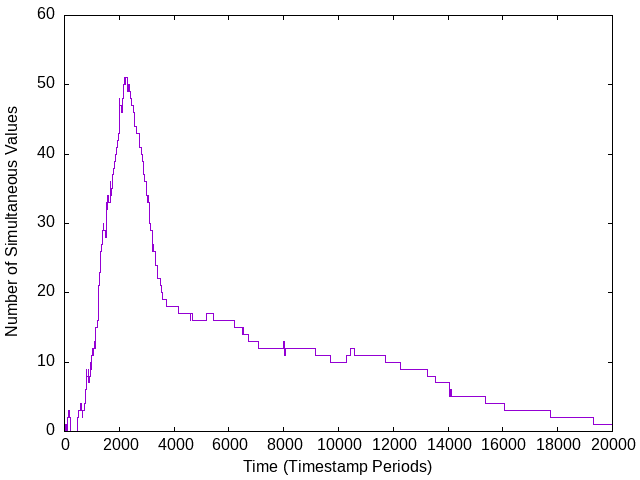
\includegraphics{coe-nvals}}
\caption{On x86, Reasonable CPUs Can Disagree}
\label{fig:On x86; Reasonable CPUs Can Disagree}
\end{center}
\end{figure}

Figure~\ref{fig:On x86; Reasonable CPUs Can Disagree}
shows the results of 79 of the systems's hardware threads simultaneously
storing their identifying integer (ranging from 0 to 78) to a shared
variable, then repeatedly doing timestamped reads from that variable.
The x-axis displays time in TSC periods, each of which is about 0.5~ns
in duration.
The y-axis shows the number of distinct opinions that the hardware
threads have as a function of time, a number that is frequently rather
larger than one.
The backwards-in-time coe link from Thread~1 to Thread~0 in
Figure~\ref{fig:IPC Diagram for coe, fre, and rfe}
is therefore entirely plausible.

\begin{figure}[tb]
\begin{center}
\resizebox{3in}{!}{\rotatebox{90}{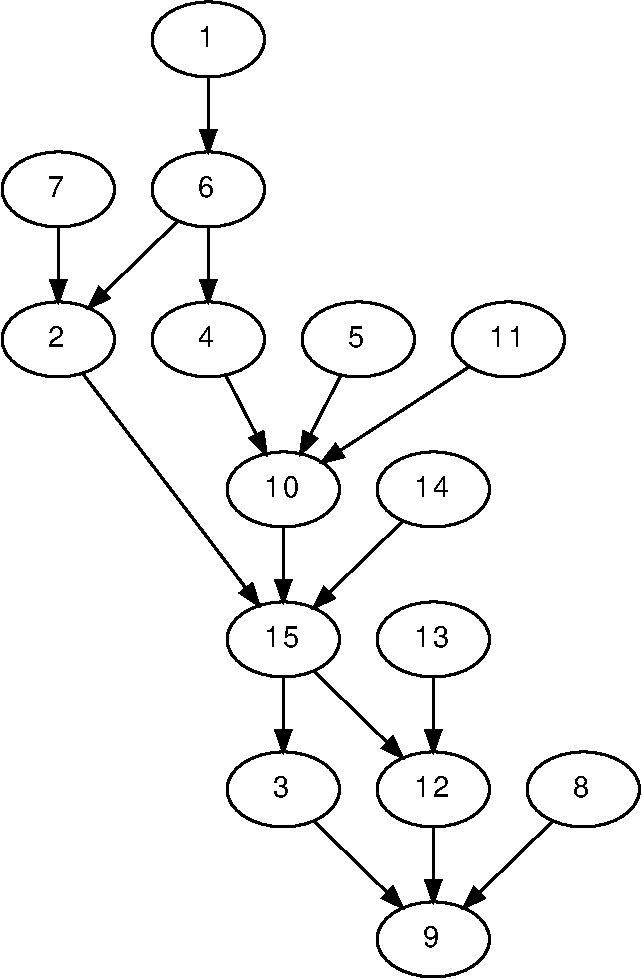
\includegraphics{store15tred}}}
\caption{On Power5, coe Links Are Also Partially Ordered}
\label{fig:On Power5, coe Links Are Also Partially Ordered}
\end{center}
\end{figure}
